\documentclass[a4paper,10pt]{book_ad}


\usepackage{poly_js}			% package for project documents
\usepackage{shortcuts_js}		% package for shortcuts 


%%%%%%%%%%%%%%%%%%%%%%%%%%%%%%%%%%%%%%%%%%%%%%%%%%
%%%%%%		Début du document 	   %%%%%%
%%%%%%%%%%%%%%%%%%%%%%%%%%%%%%%%%%%%%%%%%%%%%%%%%%




\title{Quelques outils pour démarrer en recherche en statistiques, en traitement du signal
ou apprentissage statistique}
\author{?, ?, Joseph Salmon,Yann Strozecki, Benoît Petitpas}
\date {}


\begin{document}

% \begin{comment}
% \end{comment}
\title{\vbox to 20pt{\vglue-280pt
\centerline{
\includegraphics{images/page-de-garde.pdf}
}
}
}

\author{}
\maketitle
\sloppy

%%%%%%%%%%%%%%%%%%%%%%%%%%%%%%%%%%%%%%%%%%%%%%%%%%%%%%%%%%%%%%%%%%%%%%%%%%%%%%%%%%%%%%%%%%%%%%%%%%%%%%%%%
\chapter*{Préface}
%%%%%%%%%%%%%%%%%%%%%%%%%%%%%%%%%%%%%%%%%%%%%%%%%%%%%%%%%%%%%%%%%%%%%%%%%%%%%%%%%%%%%%%%%%%%%%%%%%%%%%%%%

Voici un bref aperçu des outils (principalement numériques) pour débuter 
en recherche, dans le cadre d'un stage ou d'une thèse.
Tout ceci est purement subjectif et reflète la partialité totale et assumée des auteurs.

On aborde dans ce document des aspects techniques et pratiques :
langage de programmation, utilisation de latex pour écrire des rapports/articles/thèses.



 % change the glo to an nlo file after the makeindex, idem gls and nls
% \printnomenclature
\tableofcontents 
\newpage

\dominitoc


%%%%%%%%%%%%%%%%%%%%%%%%%%%%%%%%%%%%%%%%%%%%%%%%%%%%%%%%%%%%%%%%%%%%%%%%%%%%%%%%%%%%%%%%%%%%%%%%%%%%%%%%%
\chapter{Ressources Internet}
\minitoc

La plupart des ressources utiles sont maintenant disponibles sur le réseau,
même si la fréquentation des bibliothèques est aussi une bonne pratiques.


\section{Sites généraux}
\begin{itemize}
 \item \href{www.google.com}{Google} : 
no comment à part que paramétrer son compte
peut aider (langue par défaut, recherche détaillée avec les signes `` '' ou -).

\item \href{http://wikipedia.org/}{Wikipedia} : no comment, 
bons pour tous les niveaux, spécialement en guise d'introduction. Pour les maths,
la version française est souvent plus detaillée.

\end{itemize}




\subsection{Dictionnaire et traducteurs}

\begin{itemize}
\item \href{http://www.linguee.com/}{Linguee} : dictionnaire franco-anglais très bon, qui propose 
surtout des phrases où les mots sont contextualisés. Très précis.
\item \href{http://www.lexilogos.com/}{Lexilogos} : site référençant des dictionnaires et autres
aides (grammaire, conjugaison) pour un très grand nombre de langues. 
\item \href{https://translate.google.fr/}{Google translate} : site s'améliorant avec le temps, 
il a l'avantage d'aider à la prononciation.
\end{itemize}


\subsection{Biblioth\`eque en ligne}

\begin{itemize}

\item \href{http://catalogue-bibliotheques.upmc.fr/#focus}{Biblioth\'eque de l'UPMC} : Ressources en 
ligne et aussi disponibles sur le site de Jussieu et de Sophie-Germain.

\item des sites russes ou chinois que l'on ne saurait nommer.

\end{itemize}


\section{Sites scientifiques spécialisés}



\begin{itemize}
\item \href{http://scholar.google.com}{Scholar Google} :
Ouvrir un compte peut être une bonne idée pour augmenter sa visibilité en recherche,
et retrouver facilement ses co-auteurs sur Internet.
Il est aussi bon de paramétrer \href{http://scholar.google.com}{Scholar Google} pour
obtenir les fichiers  .bib (cf. les parties sur Latex en chapitre ... \mytodo{link})

\item \href{http://arxiv.org/}{arXiv} :
À suivre régulièrement (par exemple en consultant les flux RSS avec 
\href{https://www.newsblur.com/}{NewsBlur}). 
C'est le lieu international
où les gens déposent leurs pré-publications. C'est donc l'endroit conseillé pour faire
de même.

Potentiellement il peut être recommandé de suivre avec une certaine fréquence ce qui est soumis
chaque jour, voir profiter d'un groupe de lecture régulier pour discuter des papiers récents les plus
marquants.

\item \href{http://hal.archives-ouvertes.fr/}{Hal} : c'est l'équivalent français d'arXiv.
Les thèses françaises y sont toutes référencées.


\item \href{http://www.ams.org/mathscinet/}{Mathscinet} : référence les travaux publiés dans
des journaux de mathématiques. Utiles aussi pour trouver des fichies .bib, ainsi que les sources
des papiers. Il manque toute la partie de littérature du cote des ``computer sciences'' (sciences
computationnelles ou informatique) ainsi que les revues de type signal.
\end{itemize}





\subsection*{R\'esum\'e des sites utiles mentionés dans ce chapitre}

\begin{itemize}
\item[\color{orange_js}{$\startri$}]
\url{http://arxiv.org/}
 \item[\color{orange_js}{$\startri$}]
\url{http://scholar.google.com}
 \item[\color{orange_js}{$\startri$}]
\url{http://scholar.google.com} \item[\color{orange_js}{$\stardble$}]
\url{http://hal.archives-ouvertes.fr/}
  \item[\color{orange_js}{$\stardble$}]
\url{http://jrjohansson.github.io/}
\end{itemize}

%%%%%%%%%%%%%%%%%%%%%%%%%%%%%%%%%%%%%%%%%%%%%%%%%%%%%%%%%%%%%%%%%%%%%%%%%%%%%%%%%%%%%%%%%%%%%%%%%%%%%%%%%


%%%%%%%%%%%%%%%%%%%%%%%%%%%%%%%%%%%%%%%%%%%%%%%%%%%%%%%%%%%%%%%%%%%%%%%%%%%%%%%%%%%%%%%%%%%%%%%%%%%%%%%%%
\chapter{Bonnes pratiques	 informatiques}
\minitoc

Pour les nouveaux en programmation, il existe de nombreux langages informatiques, qui sont très 
différents les uns des autres. Nous en listerons ici un certain nombre avec des exemples d'utilisation 
optimum. Il existe en gros quatre grandes familles de code :
 %jamais été très convaincu par les familles de code on retrouve du fonctionnel et de l'objet
%dans presque totues les familles par exemple (Yann)

\begin{enumerate}
\item procédural (C, Fortran, Pascal, Basic, \ldots)
\item orienté objet (Java, C\#, Python, \ldots)
\item fonctionnel (OCaml, Lisp, \ldots)
\item logique (Prolog)
\end{enumerate}

Un site pr\'esentant des livres gratuits sur un la plupart des langages existants est
\url{https://github.com/vhf/free-programming-books/blob/master/free-programming-books.md}

Les plus utilisées sont les deux premières, en sachant qu'il existe des hybrides, notamment le C++ 
qui appartient dans sa structure même aux deux premières familles. 

\section{Programmation procédurale}

Les langages procéduraux sont une suite de routines qui s'exécutent dans l'ordre. Ce sont des ordres 
donnés à la machine qui s'exécutent pas à pas (comme une recette de cuisine).\\

Nous ne parlerons dans ce document que du C. 

\subsection{C}

C'est un langage qui n'est pas simple à prendre en main et il est \`a déconseiller sauf pour 
une chose : sa rapidité ! Pour un chercheur qui n'est pas versé dans l'art de la programmation,
il vaut mieux apprendre un langage plus moderne.

\subsubsection*{Avantages du C}
 Pour une question subtile sur le langage C, la réponse est certainement dans cette 
 \href{http://c-faq.com/}{FAQ}.
 
 
 
\begin{itemize}
\item une fois compilé, le C est très rapide, et est très proche des instructions machines,
donc si  vous devez faire du temps réel \textbf{FAITES} du C
\item le C est facilement parallélisable puisque vous contrôlez la mémoire
par exemple en utilisant \href{http://openmp.org/}{OPENMP} (possible aussi en C++)
\item le C et est un langage répandu et beaucoup de gens le comprennent
\end{itemize}

\subsubsection*{Défauts du C}

\begin{itemize}
\item il faut s'occuper de la gestion mémoire soi-même
\item coder en C est souvent plus long que dans un langage moderne
\item il n'y a pas de libraire par défaut pour les structures de données courantes ou les fonctions souvent utiles
%\item faut compiler à chaque fois
%\item c'est pas portable (ce qui marche chez vous ne marche pas chez votre voisin)
%\item c'est vieux
%\item c'est prétentieux de coder en C
\end{itemize}

\section{Programmation orientée objet}

La programmation orientée objet est difficile à définir et vous trouverez sur le net de nombreuses 
définitions possibles. En bref, c'est la même chose que précédemment mais en mieux. C'est une recette de cuisine qui se 
découpe en de nombreuses sous-recette de cuisine ultra spécialisées (comment cuire la viande,
assaisonner les légumes, faire les sauces, etc.).\\

% Conseil : n'écoutez JAMAIS les vieux briscards du code qui vous parle de VRAI programmation objet 
% ou de full OOP (oriented object programming), c'est des chieurs qu'il faut ignorer. 
% Mais il faut savoir que l'orienté objet c'est le bien le reste c'est le mal. 

Nous parlerons de deux langages uniquement : C++ et Python. 
% Me demandez pas pourquoi c'est juste que j'aime pas JAVA et que j'aime bien ces deux là! 

\subsection{C++}

Le C++ a été inventé pour faire du C orienté objet. En réalité c'est un hybride et introduit une
nouveauté : les types templétés extrêmement utiles quand on sait les utiliser.


\subsubsection*{Avantages du C++}

\begin{itemize}
\item c'est presque aussi rapide que du C mais moins quand même
\item les types templétés sont tr\`es pratiques \mytodo{pour???}
%\item les vrais, ils font du C++
\item on peut faire facilement du calcul parallèle % mais en C aussi
\end{itemize}

\subsubsection*{Défaut du C++}

\begin{itemize}
\item c'est compliqué à mettre en oeuvre
%\item faut compiler
%\item c'est presque aussi long pour coder
\item ce n'est pas portable %qu'est ce que tu entends par c'est pas portable ? 
\end{itemize}

\subsection{Python}

Python est un langage moderne, agréable d'utilisation et concis.
Il est parfaitement adapté à l'écriture de programmes dont les performances ne sont
pas importantes. Python tend à devenir un standard: ce langage est enseigné au lycée 
et en classes préparatoires (ainsi que dans les universités et les grandes \'ecoles). 

Il est donc utile de le connaître si vous avez à enseigner.

Pour apprendre Python, vous pouvez utiliser le site 
\href{http://www.codecademy.com/tracks/python}{codecademy} 
qui donne des exercices en ligne pour apprendre par l'exemple.
Le livre de Kevin Sheppard peut aussi s'avérer un compl\'ement utile: 
\href{http://www.kevinsheppard.com/images/0/09/Python_introduction.pdf}{Python Introduction}.

Enfin pour respecter un tant soit peu la syntaxe de ce langage il est bon de suivre les préceptes
de \url{http://www.python.org/dev/peps/pep-0008/} et tester la validité  de la syntaxe avec
\url{https://pypi.python.org/pypi/pep8}.

\subsubsection*{Avantages de Python}
\begin{itemize}
\item c'est simple
\item c'est réutilisable tel quel ! 
\item c'est interprété
%\item les gentils font du Python
\item c'est court à coder et à  tester
\item les tests en Python sont faciles %???
\item c'est portable
\item pip (Python Package Index):  pratique pour installer des nouveaux packages!
\item on peut faire comme du Matlab mais en gratuit ! %à expliquer plus loin
\end{itemize}

\subsubsection*{Défauts de Python}
\begin{itemize}
\item il n'y a pas les templates
\item n'importe qui peut faire n'importe quoi ! %ça n'est pas typé
\item c'est lent
\end{itemize}

\section{Dérivés et autres langages liés à des programmes}

Il existe des logiciels qui ont tellement apportés dans un domaine de recherche qu'ils sont 
indispensables dans votre travail. Notamment, si vous faites des statistiques, vous ne pourrez
 faire l'impasse d'une bonne formation en \lstinline+R+. De m\^eme en traitement du signal, 
Matlab a réussit à s'imposer comme un standard.\\

Ce sont de bons logiciels qu'il est intéressant d'utiliser, notamment dans le cas de Matlab, 
vous aurez la possibilité d'utiliser tout la base \href{http://www.mathworks.fr/matlabcentral/fileexchange}{Mathworks}.
Toutefois, il est intéressant de noter que la syntaxe de Python se reprochant de celle de Matlab, il a 
été développé en Python des bibliothèques et outils permettant de programmer en Python comme en Matlab: 
\href{http://www.numpy.org/}{numpy}, \href{http://www.scipy.org/}{scipy} et \href{http://matplotlib.org/}{matplotlib}.\\



\section{Trucs et astuces pour choisir le langage adéquate}

En fonctions de différentes problématiques il est de bon ton de savoir ce que vous devriez utiliser :

\begin{itemize}
\item Temps réel : C et c'est TOUT !!!!
\item Traitement d'image ou du son: C++ pour de grosses données, sinon Python ou Matlab
\item Vision 3D : C++ avec opencv (bien qu'imparfaite cette librairie tend à devenir classique) 
et Python si vous avez de toutes petites données
\item Computer graphics : C++ 
\item Statistiques  et machine learning : R, Python et Matlab
\end{itemize}  

\section{Bonnes pratiques en programmation scientifiques}

\subsection{Bonnes pratiques générales: DOCUMENTATION}

La première est unique règle qui compte c'est : DOCUMENTEZ!
Le reste ne peut être que des conseils superflus, DOCUMENTEZ! 

Une application, un programme, un code n'est jamais totalement perdu si 
il est accompagné d'une documentation, donc DOCUMENTEZ !\\

Il ne sert à rien de dire qu'une documentation doit contenir telle ou telle section, il faut juste 
qu'elle permette de comprendre le but du code, comment on le lance et de quoi il a besoin, DOCUMENTEZ! \\

Plus votre code sera documenté et notamment en documentation externe (README, User case, etc,.) aussi 
bien que documentation interne (commentaire du code), et plus vos papiers seront cités. 
Et plus vos papiers seront cités et plus vous pourrez obtenir un poste, DOCUMENTEZ! \\

La documentation ne sert pas seulement à la communauté, elle est avant tout là pour vous aider. 
\`A la question :"\`A quoi sert cette fonction?" une documentation permet de rappeler qu'elle
 est là pour minimiser un bidule selon un algo quelconque ! 

De plus, vous devrez forcément un jour donner votre code \`a quelqu'un (ce quelqu'un
pouvant \^etre vous m\^eme dans XXX mois, années,etc.):
la documentation permet alors \`a la personne perdue de comprendre le plus rapidement possible 
votre démarche, et à quoi servent les différentes pièces du puzzle ainsi que comment elles 
s'imbriquent. DOCUMENTEZ!

\subsubsection*{fichier README }

Tout le monde ne sera pas d'accord sur ce que doit contenir un bon README, malgré tout tentons une
 liste assez général et parfaitement subjective sur ce qu'il est bon d'y trouver : 
\begin{itemize}
\item une description détaillée du code. Permet à tout le monde de savoir quel est votre but ultime
\item une description très détaillée des entrées, sorties et paramètres. N'ayez pas peur de dire que
 vous ne traitez QUE tel cas ou que tel jeux de paramètres ou tel type d'entrée. Dans le cas où vous 
partageriez votre code et qu'il soit un tant soit peu intéressant, il se peu que la communauté s'empare 
de votre oeuvre et vous aide à l'améliorer. Mais personne ne le fera jamais pour un code non documenté 
(ou trop succinctement).
\item un lien avec votre article. TOUS vos codes doivent être en relation avec des publications qui 
devront être citées en cas d'utilisation. 
\item un manuel d'installation (le coup de compilation : ./make ...) contenant les 
dépendances AVEC leurs version (pas d'opencv tout seul par pitié : v1.16 permettra à quelqu'un de 
voir d'un seul coup d'oeil s'il va passer trois heure ou 2 minutes à compiler votre code). 
\mytodo{benoit: tu peux rendre ca lisible}
\item des exemples d'utilisation (./toto -r 65 plop.dat) et potentiellement un cas pratique, sachant
qu'un cours exemple vaut mieux qu'un long discours. Pour que
 cette partie soit intéressante et si le code est en correspondance avec une publication, mettez 
un ou deux exemples d\'ej`a développés dans votre papier.
\item Si possible un schéma de votre code (comme un arbre généalogique qui partirais de la fonction
 principale appelée par l'exécution du code vers les codes plus spécialisés)
\end{itemize}

\subsubsection*{Commentaires}

Remarquez tout d'abord qu'un simple petit commentaire en début de fonction n'est pas 
ce qu'on appelle commenter son code. 
Il faut en effet un commentaire:

\begin{itemize}
 \item pour chaque fonction,
d\'ecrivant  son but, ses entrées, ses sorties et sur sa place dans l'algorithme globale.

 \item pour chaque boucle et pour chaque calcul important. 
\end{itemize}
Exemple :
\begin{lstlisting}[style=pythonsty]
int test_tmp_of_doom(int *var, double **plop) 

/* fonction qui prend en entree un tableau de reference de 
pixel et une image de masque de covariance
 et qui renvoie l'indice du pixel contenant la plus haute 
valeur de truc */

/* Cette fonction est utile dans le calcul des extrema 
interdependant des chaines de kikoolol */

int plop=42,temp=-1;
int i=0;

for(i=0;i<plop;i++){
/* parcours des index! */
if (var[i] < plop[var[i]][i]) /*cherche + haute valeur de truc*/
/* il n'y a pas de segmentation fault car les indices sont compris 
entre 0 et 40 ... bref tout commentaire permettant de comprendre 
ce geste singulier et fort peu ordinaire */

temp = i;
}

\end{lstlisting}
Bref si vous regardez ce code, les variables sont mal nommées et rien n'a de sens MAIS les
 commentaires explique tout, sans ça, c'est le flou le plus total.

Un bon conseil est parfois de se servir des commentaires comme colonne vertébrale de votre 
code. Vous commencez d'abord par écrire les commentaires décrivant en détail votre algorithme 
PUIS vous remplissez les trous! Avec ça plus jamais aucun de problème!

\subsubsection*{Nomenclature}

Beaucoup de personnes vous donnerons de bons conseils et ne les suivront pas et soyons honnêtes, 
tout le monde a des variables qui s'appelle toto ou tmp, et c'est pas grave, si il s'agit de 
variable TRÈS locales pas de problème. 
Voici juste quelques petits conseils pour mieux choisir 
les noms:

\begin{itemize}
\item Garder la même nomenclature dans TOUT votre code (un tableau d'index qui s'appelle "index[]" 
ne doit pas s'appeler autrement ailleurs "Index[]" "var[]", et c'est la confusion assurée)
\item Choisissez comme nom de variables celles que vous utiliserez dans votre article 
(si un truc est appelé béta dans un article sur lequel vous vous fondez appelez votre put*** 
de variable "beta" et c'est tout!)
\item Éviter de mettre un coup des majuscules pour les fonctions puis en minuscules, etc.
Mettez tout en minuscule si vous n'êtes pas assez rigoureux pour garder le même typage tout 
au long de vos codes (majuscules pour fonctions, minuscules pour les variables).
\end{itemize}

\subsection{Bonnes pratiques générales dans le code}

\begin{itemize}
\item Testez chaque entrée fourni par l'utilisateur, n'oubliez jamais qu'il 
n'est là pour expérimenter les bugs laissés négligemment par 
vous! De plus cet utilisateur c'est peut-être vous dans 
le futur ! Donc il est bon de tester et de renvoyer des erreurs 
compréhensibles par tout le monde concernant les erreurs. Par exemple: 
"on a dit une image png en entrée et pas autre chose!"
\item faites un --help ou un usage dans le cas où les personnes ne rentre QUE le nom du programme : m\^eme
si cela n'arrive que quand la personne n'a pas lu le README amoureusement écrit par vos soin! Un bon
 --help peut être un beau RTFM!
\item INDENTEZ votre code
\item jamais de fonction trop longues (si ça dépasse 50 lignes de code, c'est que c'est trop
 long et que vous devriez externaliser des fonctions)
\end{itemize}

\subsubsection*{Debugger un code}

Débugger va vous prendre beaucoup de temps, incluez le dans vos prévisions, si un code doit marcher 
dans deux semaines, comptez trois semaines avec une bonne semaine de debuggage et de tests. Votre ami pour
le débuggage est simplement la fonction d'écriture sur la sortie standard (printf !). Cela vous 
permet de savoir d'où  viens le bug et souvent de mettre en avant les différents états des variables.


\subsubsection*{C/C++}

Pour éviter les problèmes allouez toujours la mémoires là où vous la libérer. Sinon, cela
fini invariablement par créer des fuites mémoires de partout. Si vous faites 
un malloc dans une fonction c'est que vous faites un free dans la MÊME fonction. \\

En C++, lorsque vous devez passer des images, matrices, structures, tableaux, string  etc ... Qui 
peuvent contenir beaucoup de données FAITES TOUJOURS un passage par référence et pas par copie :\\

int plop (std::string toto) //(copie dans la mémoire toto donc si le string fait 2Go, bah à chaque
 appel de la fonction vous recopier 2Go => pas ultime!)\\

int plop (const std::string\& toto) //utilise un pointeur sur la mémoire contenant les 2Go sans
 jamais les copier ! Le const permet d'éviter de pouvoir modifier la chaîne de caractère !\\

\subsubsection*{Python}

Lorsque vous utilisez des fonction de bibliothèques externes, éviter : \\

\begin{lstlisting}[style=pythonsty]
from lib_externe..sous_fnctn import read_image
...
read_image(input)
\end{lstlisting}
Car lorsque vous appellerez cette fonction on ne saura pas d'où elle vient, ainsi et même si 
c'est embêtant : \\

\begin{lstlisting}[style=pythonsty]
import lib_externe
...
lib_externe.fnctn.sous_fnctn.read_image(input) #c'est plus clair !
\end{lstlisting}
Le Python est un langage moins rigoureux que le C/C++ donc il vous faut l'être d'autant plus
 sinon le débuggage peut être un enfer 




\section{Langage de programmation et outils de calcul matriciel}

\mytodo{Jo, Alex: Python, Numpy, Scipy}

\mytodo{Jo, Charles, Benoit}

\subsubsection*{Matlab}

Prescrivez le FOR, il devrait être interdit en Matlab. Ce type de boucle est très lent, bref en Matlab 
faites des calcul matricielle ! Vous ne devriez d'ailleurs n'utiliser Matlab QUE pour ça !

Si vous ne connaissez rien d'autre, ce n'est pas grave mais au moins approfondissez vos connaissances 
en Matlab.  Sachez de plus qu'il existe Scipy, Matplotlib  qui sont des bibliothèques de fonctions Python 
qui permette de programmer comme en Matlab mais sans Matlab ! (Et le for est bien plus rapide 
en Python que sous Matlab)\\

Il existe une interface entre C/C++ et Matlab. C'est à dire que vous pouvez écrire des petits bout de code en C
pour les parties importantes de votre code et les intégrer grâce à des fichiers .mex dans un code matlab.

\mytodo{Jo: R, Adoop}

\subsubsection*{R} Ce langage est pour les statistiques uniquement. 
Il est pleins d'erreurs et d'inconsistances, mais
toute la communauté s'en sert (académique, banque, \textit{hedges fund}, etc.) alors parfois 
il faut y passer. 
Pour démarrer on peut conseiller \href{http://www.rstudio.com/}{Rstudio} qui a une bonne interface graphique.

\section{Calcul formel}
\mytodo{Yann: Sage,Maple, mathematica}


\subsubsection*{Sage}
Développé depuis quelques années comme une tentative de remplacement de tous les
autres logiciels de math formel,  \href{http://www.sagemath.org/}{SAGE} est un logiciel très intéressant.
C'est principalement un ensemble de programmes python qui interface tous les logiciels
libres de calcul symbolique (combinatoires, graphes, polynômes, corps \dots)
Vos programmes Sage sont en fait du Python et l'utilisation est très proche des 
autres librairie de python scientifique.
Notez que c'est un logiciel libre, activement développé notamment par des chercheurs français.

%todo parler des feuilles de calcul en ligne



%%%%%%%%%%%%%%%%%%%%%%%%%%%%%%%%%%%%%%%%%%%%%%%%%%%%%%%%%%%%%%%%%%%%%%%%%%%%%%%%%%%%%%%%%%%%%%%%%%%%%%%%%

%%%%%%%%%%%%%%%%%%%%%%%%%%%%%%%%%%%%%%%%%%%%%%%%%%%%%%%%%%%%%%%%%%%%%%%%%%%%%%%%%%%%%%%%%%%%%%%%%%%%%%%%%
\chapter{Les logiciels de gestion de version}
\minitoc
Il est rare de travailler entièrement seul dans le monde académique et écrire un document ou un code à plusieurs 
pose quelques problèmes de synchronisation et de sauvegarde. C'est pour cela qu'on utilise des logiciels de gestion de version.
Ces logiciels sont utiles également pour des projets en solitaire, car ils permettent de conserver tous les modifications
que vous apportez à un document, ce qui élimine les risques d'erreurs et de perte de votre travail. 


\section{SVN}
Ce syst\`eme est plutôt ancien, mais est souvent  disponible dans votre laboratoire, université ou école.
\mytodo{Jo , Charles}

\section{Git}
\mytodo{Alex, Yann}

Git est un logiciel de gestion de version décentralisé proposé par Linus Torvald pour
gérer le développement du noyau Linux. C'est un système extrêmement en vogue et la plupart des
 grands projets de programmation sont passés à Git. Le logiciel est parfois complexe et sans doute
 inutilement puissant pour rédiger un article à 3 ou 4. Mais, du fait de sa popularité, il y a de nombreuses
 ressources pour apprendre Git sur internet et il est très facile de monter un projet git sur un site gratuit.
 
 
 Des ressources pour apprendre Git :
 \begin{itemize}
  \item Un livre gratuit pour apprendre git \url{http://git-scm.com/book}
  \item Plusieurs sites d'apprentissage interactif par exemple  \url{http://try.github.io}
  %\item
 \end{itemize}

 
 Le mieux est de créer votre dépôt git sur un serveur de votre laboratoire si c'est possible.
 Sinon, utilisez un site comme \href{http://gitlab.org/}{Gitlab} qui permet de créer gratuitement des dépôts.
%%%%%%%%%%%%%%%%%%%%%%%%%%%%%%%%%%%%%%%%%%%%%%%%%%%%%%%%%%%%%%%%%%%%%%%%%%%%%%%%%%%%%%%%%%%%%%%%%%%%%%%%%


%%%%%%%%%%%%%%%%%%%%%%%%%%%%%%%%%%%%%%%%%%%%%%%%%%%%%%%%%%%%%%%%%%%%%%%%%%%%%%%%%%%%%%%%%%%%%%%%%%%%%%%%%
\chapter{Latex: rédiger des textes scientifiques}
\minitoc
\section{Logiciels}
Tout d'abord, il faut disposer d'un éditeur de texte et d'un compilateur.

\begin{itemize}
\item Sous Mac : installer MacTex  (éditeur + compilateur) . L'éditeur s'appelle Texshop.  
\item Sous Linux : Latex est installé de base, il vous faut juste un bon éditeur. Kile est très
 bien et suffisant
dans un premier temps. Les experts pourront utiliser Vim ou emacs. 
\item Sous Windows : installer Miktex d'abord (chercher avec un moteur de recherche) puis Texniccenter 
ou  Winshell par exemple.
\end{itemize}


\section{Format de fichiers et compilation}
En Latex, on écrit un code ``barbare'' qui sera compil\'e par un programme. Sur vos terminaux c'est Kile 
qui compilera : il faut aller dans l'onglet ``\textbf{build}'' ou ``\textbf{construire}'', puis cliquer 
sur ``\textbf{compile}''. On choisit alors le type de compilation (Latex, pdfLatex, bibtex pour la
 bibliographie \ldots). 
Si en sortie on veut un fichier ps : il faut faire ``\textbf{tex to dvi}'' puis  ``\textbf{dvi to ps}''
Si en sortie on veut un fichier pdf : il faut faire ``\textbf{pdfLatex}'' (mieux pour afficher des documents 
avec des hyperliens et des images de formats standards).

Le fichier Latex du document que vous êtes en train de lire est  disponible ici : 
\href{http://josephsalmon.eu/enseignement/M1/introlatex.tex}{ceci est un lien hypertexte}.  
Son extension est  .tex. Une fois le fichier compilé,  on obtiendra un ``joli'' document en format .pdf 
ou bien .ps. Pour visualiser le résultat il suffit d'aller dans l'onglet  ``\textbf{build}'' 
(ou constuire), choisir ``\textbf{view}`` (ou voir) puis de sélectionner ``\textbf{Viewpdf}'' 
(si l'on a fait pdfLatex).\medskip

Ceci fait, on choisit la classe de document  que l'on veut créer.  Pour les projets,  
la classe ``\textbf{article}'' est recommandée (les plus motivés qui voudraient écrire un 
livre entier pourront utiliser la classe ``\textbf{book}''). Le document commence donc par la 
commande :\medskip

\begin{lstlisting}
\documentclass[a4paper,12pt]{article}
\end{lstlisting}

Les options d'une fonction Latex sont toujours entre crochets. Ici elles déterminent le format 
(A4) du document, et définissent la taille de la police (12pt).\medskip
\section{Les Packages}

En dessous du choix de la classe on donne la définition des packages que l'on veut utiliser. 
Les packages sont des bibliothèques utilisées pour des fonctions avancées, que l'on doit charger.
 Par exemple la commande  \lstinline+\usepackage{amsmath}+ charge le package ``\textbf{asmath}'',
 qui est utile  pour écrire des symboles mathématiques. Le package ``\textbf{babel}''  est lui 
utilisé pour écrire des accents (du moins avec l'option ``\textbf{french}''). En effet, les anglophones
 n'en ont pas besoin, donc initialement Latex ne gère pas les accents. L'intérêt du package est
 donc de pallier ce manque. \medskip

Les packages sont des fichiers au format .sty. Ils sont pour la plupart déjà installés sur votre 
ordinateur (par Miktex ou Texshop). Par contre, il se peut que certains packages ne soient pas 
disponibles.  Pour les rendre utilisables pour la compilation il suffit de télécharger le fichier 
``\textbf{***.sty}''  sur internet (on les trouvera sur le site du  \href{http://www.ctan.org/}{CTAN})
  et de le placer dans le dossier où vous éditez votre fichier .tex.     \medskip

\section{Formules mathématiques et théorèmes}
On peut définir des environnements comme des théorèmes, des propositions, etc. par les commandes :\medskip
\begin{lstlisting}
\newtheorem{theorem}{Theorem}[section] 
\newtheorem{prop}[theorem]{Proposition}
\end{lstlisting}
Cela donne :

\begin{theorem}
 L'ensemble des nombres premiers est infini.
\end{theorem}
Les théorèmes  sont ainsi numérotés par Latex de manière automatique.

\begin{theorem}
 L'ensemble des nombres premiers congrus à 1 modulo 4 est infini.
\end{theorem}

\begin{proof}
 ici on ferait la démonstration ... mais  je vous la laisse en exercice.
\end{proof}



Une fois les packages définis, on peut créer des raccourcis pour les quantités qui reviennent 
souvent ou des fonctions. Ici on définit un raccourcis pour la commande qui permet de créer une
 fonction :\medskip

\lstinline+\newcommand{\nc}{\newcommand}+

\begin{rem}
 Toutes les fonctions (au sens informatique du terme) connues par Latex commencent par $\backslash$ 
(backslash) comme par exemple \lstinline+\sum+
 qui permet d'afficher le symbole de sommation $\sum_{i=1}^{4}$. 
\end{rem}


Pour les formules Mathématiques, on doit  les mettre entre deux signes 
$\$$ pour qu'elles soit interprétées comme des commandes spéciales et non comme du texte. 
Pour écrire le signe de sommation ci-dessus on écrit donc \lstinline+$\sum\_{i=1}^{4}$+ dans le 
fichier .tex. Si l'on veut afficher des calculs sur une ligne à part on peut par exemple écrire 

\[\mathcal{S}f = \sum_{k\in\mathbb{Z}} \hat{f}[k] e^{i2\pi kt/T} \] 

en mettant cette fois les formules  entre  les commandes 
\lstinline+\[+ et \lstinline+\]+. On peut aussi utiliser un environnement qui commence par la 
commande 
\lstinline+\begin{blabla}+ et finit par la commande \lstinline+\end{blabla}+. Si \lstinline+blabla=align+, 
on peut aligner des calculs facilement:
\begin{align}
 \mathcal{S}f & = \sum_{k\in\mathbb{Z}} \hat f[k] e^{i2\pi kt/T} \label{nomformule}\\
  & = \sum_{k\in\mathbb{Z}} \hat f[k] e^{i2\pi kt/T}
\end{align}

\begin{rem}
On notera que la numérotation s'est déclenchée toute seule pour les formules. 
On peut  leur donner des noms avec la commande label,  dont la syntaxe est  \lstinline+\label{nomformule}+.  
On s'y réfère plus tard dans le document  avec la commande \lstinline+\ref{nomformule}+. 
Ainsi l'ordre des équations peut être changé sans avoir besoin de re-numéroter tout un document. 
Notre première équation est donc \ref{nomformule}. 
Si l'on ne veut pas numéroter une équation,  on met une étoile à la fin de l'environnement 
(écrire \lstinline+align*+ à la place d'\lstinline+align+ par exemple).
\end{rem}



Pour un grand panel de symboles mathématiques, il suffit de regarder les raccourcis fournis par l'éditeur 
que vous utilisez ou de chercher sur Internet un lexique. Voici néanmoins quelques commandes : 
pour aller à la ligne  \lstinline+\\+, 
pour une nouvelle feuille \lstinline+\newpage+, pour les trois points  \lstinline+\ldots+\medskip
\\
On renvoit à \href{http://www.tex.ac.uk/tex-archive/info/symbols/comprehensive/symbols-a4.pdf}
{``The Comprehensive Latex Symbol List''} par Scott Pakin pour une liste exhaustive de tous les
 symboles connus.


%%%%%%%%%%%%%%%%%%%%%%%%%%%%%%%%%%%%%%%%%%%%%%%%%%%%%%%%%%%%%%%%%%%%%%%%%%%%%%%%%%%%%%%%%%%%%%%%%%%%%%%%%
\section{Organisation du document}
%%%%%%%%%%%%%%%%%%%%%%%%%%%%%%%%%%%%%%%%%%%%%%%%%%%%%%%%%%%%%%%%%%%%%%%%%%%%%%%%%%%%%%%%%%%%%%%%%%%%%%%%%


On commence par donner un titre au  fichier, le nom de l'auteur et éventuellement la date par les
 commandes suivantes :\medskip

\begin{lstlisting}
\title{Faire un rapport en Latex} 
\author{Nom} 
\date{}
\end{lstlisting}



Ensuite on commence le corps du document avec \lstinline+\begin{document}+ 
(ne pas oublier de fermer tout en bas du document par la commande \lstinline+\end{document}+). 
On insère le titre avec \lstinline+\maketitle+ et la table des matières avec \lstinline+\tableofcontents+.
La construction de la table des matières se fait automatiquement. 
Elle donne l'arborescence du document, dans l'ordre où les chapitres et sous chapitres sont donnés 
dans le fichier .tex.\medskip	


On crée  des chapitres, sous chapitres en écrivant simplement  au début d'un chapitre 
\lstinline+\chapter{Le nom du chapitre}+ 
et pour les sous-chapitres \lstinline+\section{Le nom du sous chapitre}+.  
Latex numérote tout seul les chapitres dans l'ordre où ils se présentent. 
Si l'on intervertit deux chapitres, à la prochaine compilation les numéros seront automatiquement 
échangés. Il faut parfois deux compilations pour afficher correctement la table des matières.  \medskip
 
Ceci fait vous pouvez déjà commencer à rédiger un premier document, visuellement correcte avec
 toutes les formules de mathématiques dont vous avez besoin. Au chapitre suivant on va voir 
quelques raffinements possibles pour égayer vos documents.



%%%%%%%%%%%%%%%%%%%%%%%%%%%%%%%%%%%%%%%%%%%%%%%%%%%%%%%%%%%%%%%%%%%%%%%%%%%%%%%%%%%%%%%%%%%%%%%%%%%%%%%%%
\section{Insérer une image }
%%%%%%%%%%%%%%%%%%%%%%%%%%%%%%%%%%%%%%%%%%%%%%%%%%%%%%%%%%%%%%%%%%%%%%%%%%%%%%%%%%%%%%%%%%%%%%%%%%%%%%%%%

Après avoir créé des graphiques avec Scilab, Matlab ou tout autre logiciel,  vous pouvez avoir 
envie de les insérer dans votre rapport. Cette opération est plus compliquée qu'avec un éditeur 
de texte classique. Voici le code pour insérer l'image ci-dessous : \medskip

\begin{lstlisting}
\begin{figure}[htb]
\begin{minipage}[b]{0.48\linewidth}
\centering
\centerline{\includegraphics[width=1.44\textwidth]{psnr_sig60.jpg}}
\vspace{0.1cm}
\centerline{(A) un premier graphique}
\medskip
\end{minipage}
\hfill
\begin{minipage}[b]{.48\linewidth}
\centering
\centerline{\includegraphics[width=1.44\textwidth]{psnr_sig60.jpg}}
\vspace{0.1cm}
\centerline{(B) un autre}
\end{minipage} 
\caption{Des graphiques encore des graphiques...}
\label{fig:ma_figure}
\end{figure}
\end{lstlisting} 

\medskip
\begin{figure}[htb]
\begin{minipage}[b]{0.48\linewidth}
  \centering
 \centerline{\includegraphics[width=1.44\textwidth]{srcimages/psnr_sig40}}
  \vspace{0.1cm}
  \centerline{(A) un premier graphique }\medskip
\end{minipage}
\hfill
\begin{minipage}[b]{.48\linewidth}
  \centering
 \centerline{\includegraphics[width=1.44\textwidth]{srcimages/psnr_sig60}}
  \vspace{0.1cm}
  \centerline{(B) un deuxième graphique}\medskip
\end{minipage}%

\caption{Des graphiques encore des graphiques...mais quand m\^eme le .jpg c'est bien nul	}
\label{fig:ma_figure}
\end{figure}

L'image insérée doit se trouver par défaut dans le même répertoire où se trouve le fichier .tex 
que vous écrivez. On peut d\'eclarer \`a la main les sous dossiers, ou bien cr\'eer une fois
pour toute un dossier \lstinline+images+ et d\'eclarer son chemin d'acc\`es dans le préambule
avec
\begin{lstlisting}
\graphicspath{{images/}} 
\end{lstlisting}



On pourra faire varier les paramètres de taille pour voir comment jouer sur la 
taille de l'image que l'on insère. Il existe d'autres façons d'insérer des images, mais celle-ci
 à l'avantage de bien fonctionner \ldots \medskip


En ''pdfLatex'' (version largement conseillée)  on peut insérer des images au format .jpg, .png, 
.pdf \ldots En revanche, si l'on compile pour obtenir un fichier .ps avec ``\textbf{Latex}'' il 
faut insérer des fichiers sous le format (peu connu) .eps. Les commandes en revanche ne diffèrent
 pas.\medskip

Grâce au label utilisé pour la figure, on peut se référer  à celle-ci comme pour les équations,
 par la commande \lstinline+\ref{fig:ma_figure}+. Ansi la première figure est la figure \ref{fig:ma_figure}.

\section{Liens hypertextes}

Pour ce faire il faut utiliser les packages pdftex et hyperref.
On insère un lien hypertexte par la commande 
\lstinline+\url+\nomenclature[A]{$\backslash$url}{$\backslash$url} si l'on veut écrire un lien 
hypertexte présentant le site cible. 
Par exemple on peut trouver de l'aide sur latex sur le site officiel : 
\url{http://www.ctan.org/} (la commande est \lstinline+\url{http://www.ctan.org/}+). 
Mais on peut aussi le faire avec  \lstinline+\href+, qui permet de définir n'importe quel mot 
comme lien. 
Par exemple \href{http://www.ctan.org/}{là} se trouve le site donné ci-dessus 
(avec la commande : \lstinline+\href{http://www.ctan.org/}{adresse}+).  
Les références, citations, entrées de la table des matières sont directement hypertextes 
(c.-à-d qu'on peut cliquer dessus pour aller à l'emplacement correspondant).
On pourra utiliser la ligne suivante pour définir divers packages utiles  d'un seul coup :
\begin{lstlisting}
\usepackage[pdftex,a4paper,linkcolor=test,citecolor=vertsombre,
	    colorlinks=true,pagebackref,bookmarks=true, 
	    plainpages=true,urlcolor=freeblue]{hyperref}
\end{lstlisting}

\section{Insérer un algorithme}
Plutôt que de donner un fichier de programmation, il peut être utile d'introduire dans son document
 un schéma de l'algorithme que l'on a utilisé. Pour cela, on peut choisir le package 
\lstinline+algpseudocode+

On peut alors obtenir  l'exemple suivant :\medskip 


\begin{algorithm}[h]
\KwData{les observations et leurs étiquettes $\mathcal{D}_n=\{(\mathbf{x}_i,y_i): 1\leq i \leq n\}$;
le pas de gradient: $\epsilon$; \qquad\qquad le nombre maximal d'it\'erations: $n_{\rm iter}$;}
\KwResult{$\mathbf{w}$}
initialiser (aléatoirement) $\mathbf{w}$ et  $j=0$\\
\While{$j\leq n_{\rm iter}$}{
$\mathbf{w}_{\rm{old}}\leftarrow\mathbf{w}$\\
\For{$i=1$ to $n$}{
$\mathbf{w}\leftarrow\mathbf{w}_{\rm{old}}-\epsilon 
\nabla_\mathbf{w}\ell( \hat{f}_{\mathbf{w}_{\rm{old}}}
(\mathbf x_i),y_i)$
}
$j\leftarrow j+1$
}
\caption{Perceptron}
\end{algorithm}

Les commandes utilisées sont : 

\begin{lstlisting}
\begin{algorithm}[h]
\KwData{Observations et \'etiquettes 
$\mathcal{D}_n=\{(\mathbf{x}_i,y_i): 1\leq i \leq n\}$;
le pas de gradient: $\epsilon$; \qquad\qquad 
le nombre maximal d'it\'erations: $n_{\rm iter}$;}
\KwResult{$\mathbf{w}$}
initialiser (al\'eatoirement) $\mathbf{w}$; initialiser  $j=0$\\
\While{$j\leq n_{\rm iter}$}{
$\mathbf{w}_{\rm{old}}\leftarrow\mathbf{w}$\\
\For{$i=1$ to $n$}{
$\mathbf{w}\leftarrow\mathbf{w}_{\rm{old}}-\epsilon 
\nabla_\mathbf{w}\ell( \hat{f}_{\mathbf{w}_{\rm{old}}}
(\mathbf x_i),y_i)$
}
$j\leftarrow j+1$
}
\caption{Perceptron}
\end{algorithm}
\end{lstlisting}

%% ATTENTION probl\`eme d'accent possible dans l'envuironnement lstlisting

\noindent Pour plus de détail sur ce package :

\noindent\url{www.ctan.org/get/macros/latex/contrib/algorithmicx/algorithmicx.pdf}

\section{Insertion de R et Python en latex}

Pour cela on peut regarder les packages knitr
et python


\section{Moosetex}

Pour les utilisateurs de Linux et Mac on pourra utiliser 
\href{http://www.math.u-bordeaux1.fr/~cdeledal/moosetex}{Moosetex},
principalement pour la gestion de l'insertion des images.
Un plus pour la fonction de netoyage (moosetex cleaning) \`a utiliser par exemple
avant de faire une mise \`a jour sur un system de versionnement type git ou svn.
\mytodo{Charles petit laius?}
%%%%%%%%%%%%%%%%%%%%%%%%%%%%%%%%%%%%%%%%%%%%%%%%%%%%%%%%%%%%%%%%%%%%%%%%%%%%%%%%%%%%%%%%%%%%%%%%%%%%%%%%%


%%%%%%%%%%%%%%%%%%%%%%%%%%%%%%%%%%%%%%%%%%%%%%%%%%%%%%%%%%%%%%%%%%%%%%%%%%%%%%%%%%%%%%%%%%%%%%%%%%%%%%%%%
\chapter{Communiquer sur sa recherche}
\minitoc

\section{Les presentations: Beamer, Powerpoint ou Keynote}

\mytodo{Jo}

\section{Cr\'eation graphique}
Pour les figures il est bon de connaître un
logiciel au moins pour la retouche d'image ou pour la création de schéma.
On pourra utiliser des outils ``open source'' tel  \href{http://inkscape.org/}{Inkscape}
 dont le format (vectoriel)
d'export est .svg et qui supporte l'insertion de symboles \LaTeX. 
 On peut consulter: \url{http://famelis.wordpress.com/2011/04/12/latex-and-inkscape/}
pour plus d'information.

En guise d'exemple la figure \ref{fig:smv} est produite par la commande:
\begin{lstlisting}
\begin{figure}[htb] 
\centering \def\svgwidth{200pt} 
\input{images/separateur_jo.pdf_tex} 
\caption{Marge et hyperplan s\'parateur (cas lin\'aire)} 
\label{fig:smv}
\end{figure}
\end{lstlisting}
Dans le cas de la création de ce document, on dispose dans un sous-répertoire local ``/image'',
d'un fichier \lstinline+separateur_jo.pdf_tex+ et d'un fichier \lstinline+separateur_jo.tex+
tous deux crées par \href{http://inkscape.org/}{Inkscape}.
Attention tout de m\^eme dans l'utilisation de sous dossiers,
il faut éventuellement penser \`a éditer le fichier
\lstinline+separateur_jo.tex+
et a changer la commande \lstinline+separateur_jo.pdf_tex+
par \lstinline+images/separateur_jo.pdf_tex+


\begin{figure}[htb] 
\centering \def\svgwidth{400pt} 
\input{images/separateur_jo.pdf_tex} 
\caption{Marge et hyperplan séparateur (cas linéaire)} 
\label{fig:smv}
\end{figure}


\section{Création de sites web: visibilité en ligne}
Il est des plus importants en recherche non seulement de faire des travaux de bonne qualité
mais encore de rendre ces travaux disponibles facilement sur Internet. Cela peut passer par la création
d'un site personnel sur le site de votre employeur (ou bien par la création d'un site personnel),
la création d'un compte \href{http://scholar.google.com}{Scholar Google}, ou encore la soumission de papier
sur Hal ou arXiv.
Il est également important de fournir en ligne les codes numériques qui permettent de recréer les 
expériences commentées dans un article scientifique. Cette motivation se nomme 
la recherche reproductible (\lcf par exemple le site \href{http://www.ipol.im/}{IPOL} dans le domaine
du traitement des images)  et vise à fournir comme dans les sciences expérimentales des expériences 
que l'on peut reproduire à souhait. C'est la seule manière de garantir que d'autres experimentateurs
peuvent reproduire nos propres résultats. Hélas, cette phase cruciale n'est pas toujours complètement 
prise en compte par les chercheurs de peur que quelqu'un trouve un \textit{bug} dans leur code.
De plus au cours du processus de relecture des travaux de recherches (\textit{review}) cet
aspect est parfois complètement délaissé par l'équipe éditoriale.

\begin{itemize}
 \item  html:
 \item  css:
 \item  php:
\end{itemize}


\mytodo{Jo, Benoit.}
%%%%%%%%%%%%%%%%%%%%%%%%%%%%%%%%%%%%%%%%%%%%%%%%%%%%%%%%%%%%%%%%%%%%%%%%%%%%%%%%%%%%%%%%%%%%%%%%%%%%%%%%%


%%%%%%%%%%%%%%%%%%%%%%%%%%%%%%%%%%%%%%%%%%%%%%%%%%%%%%%%%%%%%%%%%%%%%%%%%%%%%%%%%%%%%%%%%%%%%%%%%%%%%%%%%
\chapter{Bibliographie}
\minitoc


La gestion de la bibliographie est une étape importante à automatiser dans la perspective 
de la rédaction d'une thèse qui comprendra vraisemblablement plusieurs centaines de références.
Il est recommandé d'utiliser bibtex pour cela. De plus, il est bon de veiller à une harmonisation
des noms des références une bonne fois pour toute. Un conseil est de plutôt garder un fichier 
qui contient toutes les entrées que l'on fait grossir au fur et \`a mesure de ces lectures.
De plus il est bon de veiller à une connexion entre le fichier contenant les noms des références
et le dossier dans lequel on garde ces références. Sous Linux un bon candidat pour gérer
cette interconnexion est \href{http://jabref.sourceforge.net/}{Jabref}.


Pour les références bibliographiques,  il faut créer un autre fichier d'extension .bib, qui est 
l'extension des fichiers ``\textbf{bibtex}''. On le met également dans le dossier qui contient le 
fichier .tex que l'on rédige. Le fichier de la bibliographie associée à ce document est disponible
 \href{http://josephsalmon.eu/enseignement/M1/refs.bib}{là}.  On présente les articles, 
livres et autres sites webs de la façon suivante : (on peut trouver également ce type d'information
 tout rempli sur internet, comme sur le site \href{http://ams.u-strasbg.fr/mathscinet/}{MathSciNet}
 par exemple.)\medskip
\begin{lstlisting}
@inproceedings{Tsybakov03, 
  author    = {A. B. Tsybakov},
  title     = {Optimal Rates of Aggregation}, 
  booktitle = {COLT}, 
  year      = {2003}, 
  pages     = {303-313}, 
}
\end{lstlisting}

On doit alors compiler la bibliographie avec la commande bibtex. 
Selon le logiciel, ou la mani\`ere de faire,   (par exemple dans Kile) il faut aller dans l'onglet 
``\textbf{build}'' ou ``\textbf{construire}'', puis cliquer sur ``\textbf{compile}''. Le type de 
compilation est alors Bibtex.\medskip

La citation apparaît à l'endroit voulu grâce à la commande  \lstinline+\ref{nom_citation}+. 
Tout à la fin du fichier .pdf, on trouve alors  les références voulues avec tous les détails que l'on
 a précisés 
sur le document cité. 
Pour cela il faut  écrire juste avant \lstinline+\end{document}+ les commandes 
\lstinline+\bibliography{nom du fichier de la bibliographie}+
\lstinline+\bibliographystyle{alpha}+ pour que les citations apparaissent avec des lettres et l'année
 et non juste des numéros. Par exemple on peut parler de l'article \cite{Tsybakov03} ou bien du livre 
\cite{Catoni04}. Les articles non cités n'apparaissent pas. \medskip

On remarquera qu'à la fin de la bibliographie, les pages où une référence est citée apparaissent sous
 forme de liens hypertextes. C'est l'utilisation du package \lstinline+pagebackref+ qui rend cela possible.
Pour plus d'informations sur Bibtex en français : 
\href{http://www.irit.fr/~Alain.Crouzil/jaffre/LOGICIELS/LATEX_BIBTEX/bibtex1.html}{Le site de Gaël Jaffré},
\href{http://fr.wikipedia.org/wiki/BibTeX}{Wikipedia},  
et en anglais :  \href{http://www.bibtex.org/}{www.bibtex.org} 

%%%%%%%%%%%%%%%%%%%%%%%%%%%%%%%%%%%%%%%%%%%%%%%%%%%%%%%%%%%%%%%%%%%%%%%%%%%%%%%%%%%%%%%%%%%%%%%%%%%%%%%%%


%%%%%%%%%%%%%%%%%%%%%%%%%%%%%%%%%%%%%%%%%%%%%%%%%%%%%%%%%%%%%%%%%%%%%%%%%%%%%%%%%%%%%%%%%%%%%%%%%%%%%%%%%
\chapter{Publications: journaux, conférences, etc.}
\minitoc
%%%%%%%%%%%%%%%%%%%%%%%%%%%%%%%%%%%%%%%%%%%%%%%%%%%%%%%%%%%%%%%%%%%%%%%%%%%%%%%%%%%%%%%%%%%%%%%%%%%%%%%%%
\section{Journaux importants}
%%%%%%%%%%%%%%%%%%%%%%%%%%%%%%%%%%%%%%%%%%%%%%%%%%%%%%%%%%%%%%%%%%%%%%%%%%%%%%%%%%%%%%%%%%%%%%%%%%%%%%%%%


\mytodo{expliquer le fonctionnement ``à l'aveugle''}
\subsection{Statistiques}
\begin{itemize}
 \item Annals of Statistics
 \item Bernouilli
 \item Probability  Theory and Related Fields (PTRF)
 \item Statistical Science
 \item Electronic Journal of Statistics (EJS)
\end{itemize}

\subsection{Apprentissage statistique}
\begin{itemize}
 \item Journal of Machine Learning Research
 \item Machine Learning
\end{itemize}

\subsection{Vision}
\begin{itemize}
\item International Journal Computer Vision
\end{itemize}

\subsection{Traitement des images et du signal}
\begin{itemize}
 \item SIAM Imaging Science
 \item Pattern Analysis and Machine Intelligence 
 \item Trans. Image Processing
 \item Journal of Mathematical Imaging and Vision
 \item Signal Processing
\end{itemize}




%%%%%%%%%%%%%%%%%%%%%%%%%%%%%%%%%%%%%%%%%%%%%%%%%%%%%%%%%%%%%%%%%%%%%%%%%%%%%%%%%%%%%%%%%%%%%%%%%%%%%%%%%
\section{Conférences importantes}
%%%%%%%%%%%%%%%%%%%%%%%%%%%%%%%%%%%%%%%%%%%%%%%%%%%%%%%%%%%%%%%%%%%%%%%%%%%%%%%%%%%%%%%%%%%%%%%%%%%%%%%%%

\mytodo{expliquer le fonctionnement ``double aveugle'', double blind}


%%%%%%%%%%%%%%%%%%%%%%%%%%%%%%%%%%%%%%%%%%%%%%%%%%%%%%%%%%%%%%%%%%%%%%%%%%%%%%%%%%%%%%%%%%%%%%%%%%%%%%%%%
\subsection{Statistiques}

\begin{itemize}
 \item AISTATS
\end{itemize}

\subsection{Apprentissage statisitiques}
\begin{itemize}
 \item ICML, NIPS, COLT, ALT
\end{itemize}
\subsection{Vision}

\begin{itemize}
 \item ICCV, CVPR 
\end{itemize}


%%%%%%%%%%%%%%%%%%%%%%%%%%%%%%%%%%%%%%%%%%%%%%%%%%%%%%%%%%%%%%%%%%%%%%%%%%%%%%%%%%%%%%%%%%%%%%%%%%%%%%%%%
\subsection{Traitement des images et du signal}

\begin{itemize}
 \item ICIP, SSP, ICASSP, SIAM Imaging
\end{itemize}


%%%%%%%%%%%%%%%%%%%%%%%%%%%%%%%%%%%%%%%%%%%%%%%%%%%%%%%%%%%%%%%%%%%%%%%%%%%%%%%%%%%%%%%%%%%%%%%%%%%%%%%%%
\section{\'Ecoles d'\'et\' et rencontres de jeunes chercheurs}
%%%%%%%%%%%%%%%%%%%%%%%%%%%%%%%%%%%%%%%%%%%%%%%%%%%%%%%%%%%%%%%%%%%%%%%%%%%%%%%%%%%%%%%%%%%%%%%%%%%%%%%%%


%%%%%%%%%%%%%%%%%%%%%%%%%%%%%%%%%%%%%%%%%%%%%%%%%%%%%%%%%%%%%%%%%%%%%%%%%%%%%%%%%%%%%%%%%%%%%%%%%%%%%%%%%
\subsection{Statistiques}
Ce genre de rencontres permet aux jeunes chercheurs de rencontrer ses collègues d'une m\^me génération
dans une atmosphère plus détendue et plus propice aux collaborations et échanges informels que les
grandes conférences. 
\begin{itemize}

\item Les Rencontres des Jeunes Statisticiens: cet \'ev\`enement a lieu \`a Aussois (Savoie) tous les deux ans 
(ann\'ees impaires), 
g\'n\'eralement fin août. \url{http://www.sfds.asso.fr/111-Les_Rencontres_des_Jeunes_Statisticiens}

\item Colloque: "Jeunes Probabilistes et Statisticiens" qui a lieu tous les deux ans \'egalement ((ann\'ees paires)
et permet de rencontrer un public plus large ouvert aussi aux probabilistes. \url{http://jps.math.cnrs.fr/2014/}

\end{itemize}


%%%%%%%%%%%%%%%%%%%%%%%%%%%%%%%%%%%%%%%%%%%%%%%%%%%%%%%%%%%%%%%%%%%%%%%%%%%%%%%%%%%%%%%%%%%%%%%%%%%%%%%%%
\subsection{Traitement des images et du signal}



\begin{itemize}
\item \'Ecole d'été de Peyresq, rendev-vous annuel:
\url{http://www.gretsi.fr/ecole-d-ete-de-peyresq.php}
\end{itemize}


%%%%%%%%%%%%%%%%%%%%%%%%%%%%%%%%%%%%%%%%%%%%%%%%%%%%%%%%%%%%%%%%%%%%%%%%%%%%%%%%%%%%%%%%%%%%%%%%%%%%%%%%%
\section{Séminaires (parisiens)}
%%%%%%%%%%%%%%%%%%%%%%%%%%%%%%%%%%%%%%%%%%%%%%%%%%%%%%%%%%%%%%%%%%%%%%%%%%%%%%%%%%%%%%%%%%%%%%%%%%%%%%%%%

%%%%%%%%%%%%%%%%%%%%%%%%%%%%%%%%%%%%%%%%%%%%%%%%%%%%%%%%%%%%%%%%%%%%%%%%%%%%%%%%%%%%%%%%%%%%%%%%%%%%%%%%%
\subsection{Statistiques}

\begin{itemize}
 \item Le lundi après midi, une fois par mois:
 \href{https://sites.google.com/site/semstats/}{Séminaire Parisien de Statistique}
 \item Le lundi et jeudi, deux fois par mois:  
\href{https://sites.google.com/site/smileinparis/home}{SMILE (Statistical Machine Learning in Paris)}
 \item Le lundi: 
\href{http://certis.enpc.fr/~dalalyan/seminar.html}{Séminaire statistique de l'ENSAE-CREST}
 \item Le lundi une fois par mois environ \`a l'universit\'e Paris Diderot-Paris 7:  
\href{http://dominiquepicard.blogspot.fr/p/seminaire-point-de-vue.html}{Point de vue}
\end{itemize}



%%%%%%%%%%%%%%%%%%%%%%%%%%%%%%%%%%%%%%%%%%%%%%%%%%%%%%%%%%%%%%%%%%%%%%%%%%%%%%%%%%%%%%%%%%%%%%%%%%%%%%%%%
\subsection{Images}
\begin{itemize}
 
 \item Le vendredi matin, une fois par mois:
 \href{http://w3.mi.parisdescartes.fr/map5/-Groupe-de-travail-Modelisation-}
{Groupe de travail Modélisation numérique et Images
}
\end{itemize}

%%%%%%%%%%%%%%%%%%%%%%%%%%%%%%%%%%%%%%%%%%%%%%%%%%%%%%%%%%%%%%%%%%%%%%%%%%%%%%%%%%%%%%%%%%%%%%%%%%%%%%%%%


%%%%%%%%%%%%%%%%%%%%%%%%%%%%%%%%%%%%%%%%%%%%%%%%%%%%%%%%%%%%%%%%%%%%%%%%%%%%%%%%%%%%%%%%%%%%%%%%%%%%%%%%%
\chapter{Recrutement des chercheurs et enseignants chercheurs}
\minitoc



\href{http://guilde.jeunes-chercheurs.org/}{la guilde du doctorant}: France

\href{http://postes.smai.emath.fr/}{Opération postes}: France

\href{https://www.galaxie.enseignementsup-recherche.gouv.fr/ensup/candidats.html}{Galaxie}: France

\href{http://www.phds.org/}{Phds.org}: international

\href{https://www.mathjobs.org/jobs}{MathJobs}: international

\href{http://notable.math.ucdavis.edu/wiki/Mathematics_Jobs_Wiki}{Mathematics Jobs Wiki} principalement
pour les \'Etats-Unis

\section{Post-doc}
\mytodo{Jo,Charles}

\section{Chercheurs: concours CNRS, Inria}
\mytodo{Charles: CNRS, INRIA}

\section{Maître de conférences (France)}
\mytodo{Jo,Yann,}

\section{Assistant Professor (France)}
\mytodo{Jo,Yann,Alex}
%%%%%%%%%%%%%%%%%%%%%%%%%%%%%%%%%%%%%%%%%%%%%%%%%%%%%%%%%%%%%%%%%%%%%%%%%%%%%%%%%%%%%%%%%%%%%%%%%%%%%%%%%


%%%%%%%%%%%%%%%%%%%%%%%%%%%%%%%%%%%%%%%%%%%%%%%%%%%%%%%%%%%%%%%%%%%%%%%%%%%%%%%%%%%%%%%%%%%%%%%%%%%%%%%%%
\appendix
\chapter{Annexe}
Cette partie est créee avec la commande \lstinline+\appendix+, 
on crée un chapitre à part dans lequel la numération est distincte du corps du document.
\chapter{Programmes}
Ici on peut mettre les programmes informatiques que l'on a rédigés \ldots
\section{Démonstrations }
Ici on peut mettre en appendice des calculs trop longs pour le corps du texte

\chapter{Remerciements}
Merci \`a G\'erard Blanchet pour le document  de la Figure \ref{fig:smv}
illustrant l'intérêt de Inkscape. Merci \'egalement \`a Arnak Dalalyan
d'avoir mis au point le fichier .cls utilisé pour ce document.
%%%%%%%%%%%%%%%%%%%%%%%%%%%%%%%%%%%%%%%%%%%%%%%%%%%%%%%%%%%%%%%%%%%%%%%%%%%%%%%%%%%%%%%%%%%%%%%%%%%%%%%%%


%%%%%%%%%%%%%%%%%%%%%%%%%%%%%%%%%%%%%%%%%%%%%%%%%%%%%%%%%%%%%%%%%%%%%%%%%%%%%%%%%%%%%%%%%%%%%%%%%%%%%%%%%
\printnomenclature
\clearpage
% \addcontentsline{toc}{chapter}{Bibliographie}
\bibliographystyle{plainnat}
%\bibliographystyle{plain}
\bibliography{refs}
%%%%%%%%%%%%%%%%%%%%%%%%%%%%%%%%%%%%%%%%%%%%%%%%%%%%%%%%%%%%%%%%%%%%%%%%%%%%%%%%%%%%%%%%%%%%%%%%%%%%%%%%%
\end{document}


